% ##QuantumErrorCorrection ##Decoding ##SurfaceCode ##CorrelatedErrors 
\documentclass[a4paper, english]{scrartcl}
\usepackage[utf8]{inputenc}
\usepackage{amsmath}
\usepackage{amsfonts}
\usepackage{amssymb}
\usepackage{babel}
\usepackage[cm]{fullpage}
\usepackage{float}
\usepackage{graphicx}
\usepackage{helvet}
\usepackage{hyperref}
\usepackage{mathtools}
\usepackage{nicefrac}
\usepackage{tikz}
\usepackage{pgfplots}
\usepackage{placeins}
\usepackage{verbatim}
\usepackage{xcolor}
\definecolor{gr}{gray}{0.9}
\renewcommand{\familydefault}{\sfdefault}
\title{Quantum Error Correction}
\subtitle{Correlated Decoding as Bilinear Programming}
\author{Ben Criger}
\date{\today}
%    Q-circuit version 2
%    Copyright (C) 2004  Steve Flammia & Bryan Eastin
%    Last modified on: 9/16/2011
%
%    This program is free software; you can redistribute it and/or modify
%    it under the terms of the GNU General Public License as published by
%    the Free Software Foundation; either version 2 of the License, or
%    (at your option) any later version.
%
%    This program is distributed in the hope that it will be useful,
%    but WITHOUT ANY WARRANTY; without even the implied warranty of
%    MERCHANTABILITY or FITNESS FOR A PARTICULAR PURPOSE.  See the
%    GNU General Public License for more details.
%
%    You should have received a copy of the GNU General Public License
%    along with this program; if not, write to the Free Software
%    Foundation, Inc., 59 Temple Place, Suite 330, Boston, MA  02111-1307  USA

% Thanks to the Xy-pic guys, Kristoffer H Rose, Ross Moore, and Daniel Müllner,
% for their help in making Qcircuit work with Xy-pic version 3.8.  
% Thanks also to Dave Clader, Andrew Childs, Rafael Possignolo, Tyson Williams,
% Sergio Boixo, Cris Moore, Jonas Anderson, and Stephan Mertens for helping us test 
% and/or develop the new version.

\usepackage{xy}
\xyoption{matrix}
\xyoption{frame}
\xyoption{arrow}
\xyoption{arc}

\usepackage{ifpdf}
\ifpdf
\else
\PackageWarningNoLine{Qcircuit}{Qcircuit is loading in Postscript mode.  The Xy-pic options ps and dvips will be loaded.  If you wish to use other Postscript drivers for Xy-pic, you must modify the code in Qcircuit.tex}
%    The following options load the drivers most commonly required to
%    get proper Postscript output from Xy-pic.  Should these fail to work,
%    try replacing the following two lines with some of the other options
%    given in the Xy-pic reference manual.
\xyoption{ps}
\xyoption{dvips}
\fi

% The following resets Xy-pic matrix alignment to the pre-3.8 default, as
% required by Qcircuit.
\entrymodifiers={!C\entrybox}

\newcommand{\bra}[1]{{\left\langle{#1}\right\vert}}
\newcommand{\ket}[1]{{\left\vert{#1}\right\rangle}}
    % Defines Dirac notation. %7/5/07 added extra braces so that the commands will work in subscripts.
\newcommand{\qw}[1][-1]{\ar @{-} [0,#1]}
    % Defines a wire that connects horizontally.  By default it connects to the object on the left of the current object.
    % WARNING: Wire commands must appear after the gate in any given entry.
\newcommand{\qwx}[1][-1]{\ar @{-} [#1,0]}
    % Defines a wire that connects vertically.  By default it connects to the object above the current object.
    % WARNING: Wire commands must appear after the gate in any given entry.
\newcommand{\cw}[1][-1]{\ar @{=} [0,#1]}
    % Defines a classical wire that connects horizontally.  By default it connects to the object on the left of the current object.
    % WARNING: Wire commands must appear after the gate in any given entry.
\newcommand{\cwx}[1][-1]{\ar @{=} [#1,0]}
    % Defines a classical wire that connects vertically.  By default it connects to the object above the current object.
    % WARNING: Wire commands must appear after the gate in any given entry.
\newcommand{\gate}[1]{*+<.6em>{#1} \POS ="i","i"+UR;"i"+UL **\dir{-};"i"+DL **\dir{-};"i"+DR **\dir{-};"i"+UR **\dir{-},"i" \qw}
    % Boxes the argument, making a gate.
\newcommand{\meter}{*=<1.8em,1.4em>{\xy ="j","j"-<.778em,.322em>;{"j"+<.778em,-.322em> \ellipse ur,_{}},"j"-<0em,.4em>;p+<.5em,.9em> **\dir{-},"j"+<2.2em,2.2em>*{},"j"-<2.2em,2.2em>*{} \endxy} \POS ="i","i"+UR;"i"+UL **\dir{-};"i"+DL **\dir{-};"i"+DR **\dir{-};"i"+UR **\dir{-},"i" \qw}
    % Inserts a measurement meter.
    % In case you're wondering, the constants .778em and .322em specify
    % one quarter of a circle with radius 1.1em.
    % The points added at + and - <2.2em,2.2em> are there to strech the
    % canvas, ensuring that the size is unaffected by erratic spacing issues
    % with the arc.
\newcommand{\measure}[1]{*+[F-:<.9em>]{#1} \qw}
    % Inserts a measurement bubble with user defined text.
\newcommand{\measuretab}[1]{*{\xy*+<.6em>{#1}="e";"e"+UL;"e"+UR **\dir{-};"e"+DR **\dir{-};"e"+DL **\dir{-};"e"+LC-<.5em,0em> **\dir{-};"e"+UL **\dir{-} \endxy} \qw}
    % Inserts a measurement tab with user defined text.
\newcommand{\measureD}[1]{*{\xy*+=<0em,.1em>{#1}="e";"e"+UR+<0em,.25em>;"e"+UL+<-.5em,.25em> **\dir{-};"e"+DL+<-.5em,-.25em> **\dir{-};"e"+DR+<0em,-.25em> **\dir{-};{"e"+UR+<0em,.25em>\ellipse^{}};"e"+C:,+(0,1)*{} \endxy} \qw}
    % Inserts a D-shaped measurement gate with user defined text.
\newcommand{\multimeasure}[2]{*+<1em,.9em>{\hphantom{#2}} \qw \POS[0,0].[#1,0];p !C *{#2},p \drop\frm<.9em>{-}}
    % Draws a multiple qubit measurement bubble starting at the current position and spanning #1 additional gates below.
    % #2 gives the label for the gate.
    % You must use an argument of the same width as #2 in \ghost for the wires to connect properly on the lower lines.
\newcommand{\multimeasureD}[2]{*+<1em,.9em>{\hphantom{#2}} \POS [0,0]="i",[0,0].[#1,0]="e",!C *{#2},"e"+UR-<.8em,0em>;"e"+UL **\dir{-};"e"+DL **\dir{-};"e"+DR+<-.8em,0em> **\dir{-};{"e"+DR+<0em,.8em>\ellipse^{}};"e"+UR+<0em,-.8em> **\dir{-};{"e"+UR-<.8em,0em>\ellipse^{}},"i" \qw}
    % Draws a multiple qubit D-shaped measurement gate starting at the current position and spanning #1 additional gates below.
    % #2 gives the label for the gate.
    % You must use an argument of the same width as #2 in \ghost for the wires to connect properly on the lower lines.
\newcommand{\control}{*!<0em,.025em>-=-<.2em>{\bullet}}
    % Inserts an unconnected control.
\newcommand{\controlo}{*+<.01em>{\xy -<.095em>*\xycircle<.19em>{} \endxy}}
    % Inserts a unconnected control-on-0.
\newcommand{\ctrl}[1]{\control \qwx[#1] \qw}
    % Inserts a control and connects it to the object #1 wires below.
\newcommand{\ctrlo}[1]{\controlo \qwx[#1] \qw}
    % Inserts a control-on-0 and connects it to the object #1 wires below.
\newcommand{\targ}{*+<.02em,.02em>{\xy ="i","i"-<.39em,0em>;"i"+<.39em,0em> **\dir{-}, "i"-<0em,.39em>;"i"+<0em,.39em> **\dir{-},"i"*\xycircle<.4em>{} \endxy} \qw}
    % Inserts a CNOT target.
\newcommand{\qswap}{*=<0em>{\times} \qw}
    % Inserts half a swap gate.
    % Must be connected to the other swap with \qwx.
\newcommand{\multigate}[2]{*+<1em,.9em>{\hphantom{#2}} \POS [0,0]="i",[0,0].[#1,0]="e",!C *{#2},"e"+UR;"e"+UL **\dir{-};"e"+DL **\dir{-};"e"+DR **\dir{-};"e"+UR **\dir{-},"i" \qw}
    % Draws a multiple qubit gate starting at the current position and spanning #1 additional gates below.
    % #2 gives the label for the gate.
    % You must use an argument of the same width as #2 in \ghost for the wires to connect properly on the lower lines.
\newcommand{\ghost}[1]{*+<1em,.9em>{\hphantom{#1}} \qw}
    % Leaves space for \multigate on wires other than the one on which \multigate appears.  Without this command wires will cross your gate.
    % #1 should match the second argument in the corresponding \multigate.
\newcommand{\push}[1]{*{#1}}
    % Inserts #1, overriding the default that causes entries to have zero size.  This command takes the place of a gate.
    % Like a gate, it must precede any wire commands.
    % \push is useful for forcing columns apart.
    % NOTE: It might be useful to know that a gate is about 1.3 times the height of its contents.  I.e. \gate{M} is 1.3em tall.
    % WARNING: \push must appear before any wire commands and may not appear in an entry with a gate or label.
\newcommand{\gategroup}[6]{\POS"#1,#2"."#3,#2"."#1,#4"."#3,#4"!C*+<#5>\frm{#6}}
    % Constructs a box or bracket enclosing the square block spanning rows #1-#3 and columns=#2-#4.
    % The block is given a margin #5/2, so #5 should be a valid length.
    % #6 can take the following arguments -- or . or _\} or ^\} or \{ or \} or _) or ^) or ( or ) where the first two options yield dashed and
    % dotted boxes respectively, and the last eight options yield bottom, top, left, and right braces of the curly or normal variety.  See the Xy-pic reference manual for more options.
    % \gategroup can appear at the end of any gate entry, but it's good form to pick either the last entry or one of the corner gates.
    % BUG: \gategroup uses the four corner gates to determine the size of the bounding box.  Other gates may stick out of that box.  See \prop.

\newcommand{\rstick}[1]{*!L!<-.5em,0em>=<0em>{#1}}
    % Centers the left side of #1 in the cell.  Intended for lining up wire labels.  Note that non-gates have default size zero.
\newcommand{\lstick}[1]{*!R!<.5em,0em>=<0em>{#1}}
    % Centers the right side of #1 in the cell.  Intended for lining up wire labels.  Note that non-gates have default size zero.
\newcommand{\ustick}[1]{*!D!<0em,-.5em>=<0em>{#1}}
    % Centers the bottom of #1 in the cell.  Intended for lining up wire labels.  Note that non-gates have default size zero.
\newcommand{\dstick}[1]{*!U!<0em,.5em>=<0em>{#1}}
    % Centers the top of #1 in the cell.  Intended for lining up wire labels.  Note that non-gates have default size zero.
\newcommand{\Qcircuit}{\xymatrix @*=<0em>}
    % Defines \Qcircuit as an \xymatrix with entries of default size 0em.
\newcommand{\link}[2]{\ar @{-} [#1,#2]}
    % Draws a wire or connecting line to the element #1 rows down and #2 columns forward.
\newcommand{\pureghost}[1]{*+<1em,.9em>{\hphantom{#1}}}
    % Same as \ghost except it omits the wire leading to the left. 

\usepackage{amsmath}
\usepackage{bbold}
\usepackage{color}
\usepackage{stmaryrd}
\usepackage{calc}
\usepackage{verbatim}
\usepackage{mathtools}
\usepackage{xspace}
\DeclarePairedDelimiter{\ceil}{\lceil}{\rceil}
\DeclarePairedDelimiter{\floor}{\lfloor}{\rfloor}
\usepackage{tikz}
\usetikzlibrary{calc}
\providecommand{\polygon}[2]{%
  let \n{len} = {2*#2*tan(360/(2*#1))} in
 ++(0,-#2) ++(\n{len}/2,0) \foreach \x in {1,...,#1} { -- ++(\x*360/#1:\n{len})}}

\DeclareMathOperator\erf{erf}
\DeclareMathOperator\erfc{erfc}

\newsavebox\CBox
\newcommand\hcancel[2][0.5pt]{%
  \ifmmode\sbox\CBox{$#2$}\else\sbox\CBox{#2}\fi%
  \makebox[0pt][l]{\usebox\CBox}%  
  \rule[0.5\ht\CBox-#1/2]{\wd\CBox}{#1}}

\providecommand{\drv}[1]{\dfrac{\partial }{\partial #1}}
\providecommand{\drf}[2]{\dfrac{\partial #1}{\partial #2}}
\providecommand{\ddrf}[3]{\dfrac{\partial^2 #1}{\partial #2 \partial #3}}

\providecommand{\tr}{\mathrm{tr}}
 
\providecommand{\ket}[1]{\left \vert #1 \right \rangle}
\providecommand{\bra}[1]{\left \langle #1 \right \vert}
\providecommand{\braket}[2]{\left \langle #1 \left \vert #2 \right. \right \rangle}
\providecommand{\angles}[1]{\left \langle #1 \right \rangle}
\providecommand{\elem}[3]{\left \langle #1 \left \vert \vphantom{#1#2#3} #2 \right \vert #3 \right \rangle}
\providecommand{\delem}[2]{\left \langle #1 \left \vert \vphantom{#1#2} #2 \right \vert #1 \right \rangle}
\providecommand{\ketbra}[2]{\ket{#1} \! \bra{#2}}
\providecommand{\proj}[1]{\ketbra{#1}{#1}}
\providecommand{\twonorm}[1]{\| #1 \|_2}
\providecommand{\abs}[1]{\left \vert #1 \right \vert}
\providecommand{\set}[1]{\left \lbrace #1 \right \rbrace}
\providecommand{\group}[1]{\left \langle #1 \right \rangle}
\providecommand{\red}[1]{\textcolor[rgb]{0.5,0,0}{#1}}
\providecommand{\blue}[1]{\textcolor[rgb]{0,0,0.5}{#1}}
\providecommand{\green}[1]{\textcolor[rgb]{0,0.5,0}{#1}}
\providecommand{\conjecture}[1]{\red{#1 (check this).}}
\providecommand{\future}[1]{\green{#1 (do this later).}}
\providecommand{\id}{\hat{\mathbb{1}}}
\providecommand{\com}[2]{\left[#1,\,#2 \right]}
\providecommand{\acom}[2]{\left \lbrace #1,\,#2 \right \rbrace}
\providecommand{\diss}[2]{\mathcal{D}\left[ #1 \right]\left( #2 \right)}
\providecommand{\meas}[2]{\mathcal{M}\left[ #1 \right]\left( #2 \right)}
\providecommand{\lindtwo}[2]{ #1 #2 #1^{\dagger} - \dfrac{1}{2} \left \lbrace #1^{\dagger} #1,\,#2 \right \rbrace }
\providecommand{\lindthree}[3]{ #1 #2 #3 - \dfrac{1}{2} \acom{#3 #1}{#2} }
\providecommand{\lindfour}[4]{ #1 #2 #3 - \dfrac{1}{2} \acom{#4}{#2} }
\providecommand{\meastwo}[2]{ #1 #2 + #2 #1^{\dagger} - \tr \left( #1 #2 + #2 #1^{\dagger} \right) #2 }
\providecommand{\tenscom}[4]{\com{#1\otimes #2}{#3 \otimes #4}=\dfrac{1}{2}\left( \com{#1}{#3} \otimes \acom{#2}{#4} + \acom{#1}{#3} \otimes \com{#2}{#4} \right)}
\providecommand{\tenscomsimple}[4]{\com{#1\otimes #2}{#3 \otimes #4} = #1 #3 \otimes \com{#2}{#4} + \com{#1}{#3} \otimes  #4 #2}
\providecommand{\tensacom}[4]{\acom{#1\otimes #2}{#3 \otimes #4}=\dfrac{1}{2}\left( \com{#1}{#3} \otimes \com{#2}{#4} + \acom{#1}{#3} \otimes \acom{#2}{#4} \right)}
\providecommand{\trace}[1]{\mathrm{tr} \left( #1 \right)}
\providecommand{\comp}{\mathop{\bigcirc}}
\providecommand{\swap}{\textsc{swap}\xspace}
\providecommand{\cnot}{\textsc{cnot}\xspace}
\providecommand{\col}{\textrm{col}}
\providecommand{\qec}[3]{\llbracket #1,\,#2,\,#3 \rrbracket}
\providecommand{\set}[1]{\left \lbrace #1 \right \rbrace}
\renewcommand{\Im}{\textrm{Im}}
\renewcommand{\Re}{\textrm{Re}}
\providecommand{\lind}{\mathcal{L}}
\providecommand{\norm}[2]{\left \vert \left \vert #2 \right \vert \right \vert_{#1}}
\providecommand{\supp}[1]{\mathrm{supp}\left( #1 \right)}
\providecommand{\given}{\, \middle \vert \,}
\providecommand{\suchthat}{\, \middle \vert \,}
\providecommand{\diag}[1]{\mathrm{diag}\left( #1 \right)}
\providecommand{\ct}{^{\dagger}}

\providecommand{\norm}[1]{\left\Vert #1 \right\Vert} %only works with amsmath

\providecommand{\ncrit}{$n_{\textrm{crit}}$\xspace}

\makeatletter
\providecommand{\pr}[2]{p\left(#1\,\middle|\,#2\right)}
\newcommand{\pushright}[1]{\ifmeasuring@#1\else\omit\hfill$\displaystyle#1$\fi\ignorespaces}
\newcommand{\pushleft}[1]{\ifmeasuring@#1\else\omit$\displaystyle#1$\hfill\fi\ignorespaces}
\makeatother
\newlength\figureheight
\newlength\figurewidth
\setlength\figureheight{7cm}
\setlength\figurewidth{12cm}

\providecommand{\cnot}{\textsc{cnot}}

\usetikzlibrary{decorations.pathreplacing, decorations.pathmorphing, shapes.geometric, calc}

\begin{document}
\maketitle
\section{Introduction}
The toric code is a popular 2D nearest-neighbour LDPC code whose decoding can be efficiently accomplished by minimum-weight perfect matching. 
Qubits are placed on the edges of a square tiling of a 2D torus, and are subjected to one of three errors, with labels $X$, $Y$ and $Z$:
\begin{figure}[!h]
\centering
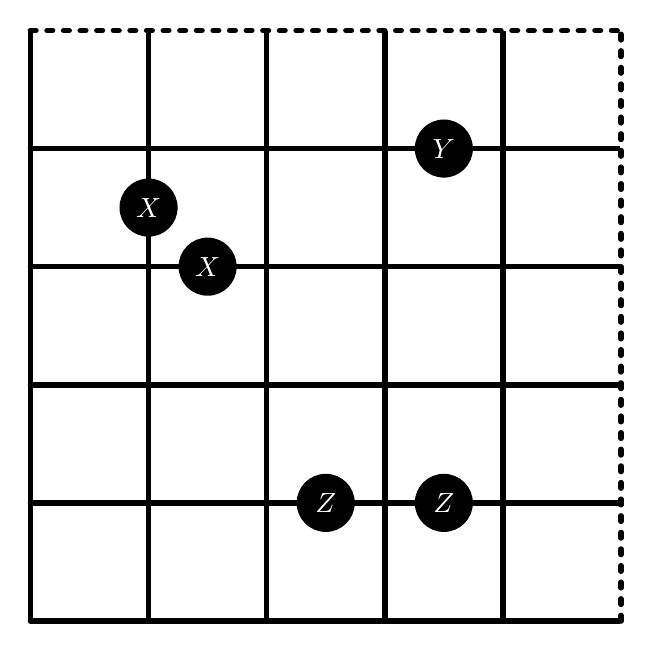
\begin{tikzpicture}[scale=0.75]
\draw[step=2, line width = 2pt, loosely dotted, line cap=round, line join=round] (0,0) grid (10,10);
\draw[step=2, line width = 2pt] (0,0) grid (9.99,9.99);
\foreach \x/\y/\err in {5/2/$Z$, 7/2/$Z$, 3/6/$X$, 2/7/$X$, 7/8/$Y$}{
\fill[black] (\x,\y) circle(14pt);
\node[white] at (\x,\y){\err};
}
\end{tikzpicture}
\caption{5-by-5 toric code lattice with an error configuration.
Qubits are supported on each edge, of which there are 50.
Five of these qubits have been subject to an error, drawn from the set $\set{X,\,Y,\,Z}$. 
Edges with no marker are not subject to error. 
Dotted edges indicate `wrapping around' the boundary to create a torus.}
\end{figure}

The parity checks of this code respond to $X$ and $Z$ errors, indicating when an odd number of $X$ errors surround a tile, and an odd number of $Z$ errors surround a vertex:
\begin{figure}[!h]
\centering
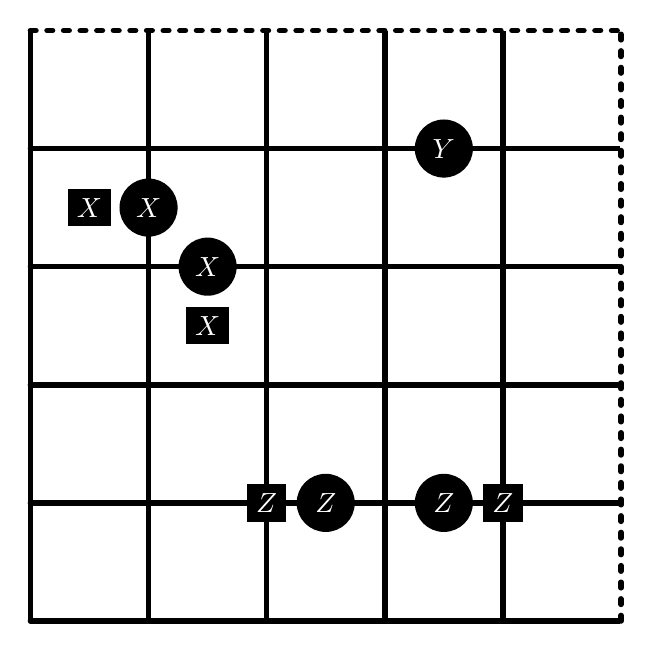
\begin{tikzpicture}[scale=0.75]
\draw[step=2, line width = 2pt, loosely dotted, line cap=round, line join=round] (0,0) grid (10,10);
\draw[step=2, line width = 2pt] (0,0) grid (9.99,9.99);
\foreach \x/\y/\err in {5/2/$Z$, 7/2/$Z$, 3/6/$X$, 2/7/$X$, 7/8/$Y$}{
\fill[black] (\x,\y) circle(14pt);
\node[white] at (\x,\y){\err};
}
\foreach \x/\y/\synd in {4/2/$Z$, 8/2/$Z$, 3/5/$X$, 1/7/$X$}{
\node[fill=black] at (\x,\y){\textcolor{white}{\synd}};
}
\end{tikzpicture}
\caption{Syndromes corresponding to $X$ and $Z$ errors.}
\end{figure}
\FloatBarrier
One thing to notice about these syndromes is that, if a continuous chain of errors of the either $X$ or $Z$ type appears on the lattice, two syndromes will appear at the endpoints of the chain.
If only $X$ and $Z$ errors occur, then, the assignment of an error to a given syndrome in the toric code can be reduced to minimum-weight perfect matching, since the probability of an error chain can be expressed as a function of the distance between the syndromes.

If $Y$ errors could be independently detected and decoded in the same fashion, we'd be done. 
The problem is that, due to Quantum Code Technicalities\textsuperscript{\textregistered}, a $Y$ error produces a pair of $X$ \emph{and} $Z$ syndromes:
\begin{figure}[!h]
\centering
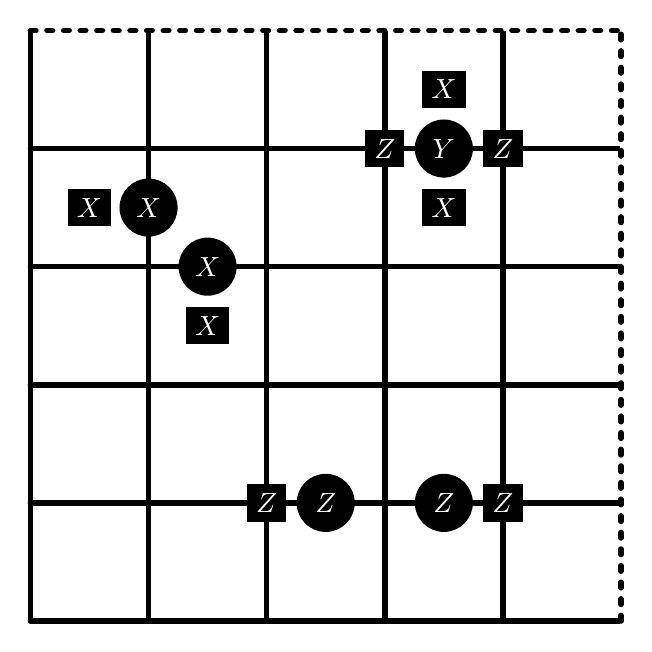
\begin{tikzpicture}[scale=0.75]
\draw[step=2, line width = 2pt, loosely dotted, line cap=round, line join=round] (0,0) grid (10,10);
\draw[step=2, line width = 2pt] (0,0) grid (9.99,9.99);
\foreach \x/\y/\err in {5/2/$Z$, 7/2/$Z$, 3/6/$X$, 2/7/$X$, 7/8/$Y$}{
\fill[black] (\x,\y) circle(14pt);
\node[white] at (\x,\y){\err};
}
\foreach \x/\y/\synd in {4/2/$Z$, 8/2/$Z$, 3/5/$X$, 1/7/$X$, 7/9/$X$, 7/7/$X$, 6/8/$Z$, 8/8/$Z$}{
\node[fill=black] at (\x,\y){\textcolor{white}{\synd}};
}
\end{tikzpicture}
\caption{Syndromes corresponding to $X$, $Y$ and $Z$ errors.}
\end{figure}

Our decoding problem is made more difficult by this, though decent performance can still be obtained by assuming that $Y$ errors occur with probability $\sim p^2$ (this works because a $Y$ error is the result of an $X$ and a $Z$ error occurring on the same qubit, bu we don't need to get into it), and decoding the $X$ and $Z$ syndromes independently.
This leaves a gap in the decoder's performance, that we're hoping to fix.
 
Existing approaches for this problem \cite{Fowler, DelfosseTillich} rely on \emph{reweighting}, adjusting the edge weights in an $X$ syndrome graph based on where $Z$ errors have been inferred, or vice versa. 
These weights are derived from \emph{conditional} probabilities, treating $p(Y)=p\left(X\given Z \right)$ or $p\left(Z\given X \right)$.

I have beef with this:
\begin{itemize}
\item It multiplies runtime by a factor of at least two, since the matching problem must be solved for one graph before the result can be applied to the other. 
This factor may be larger if we iterate, using each matching to reweight the other graph until convergence.
\item Performance can, in principle, depend on which graph we match first. It may be the case that both orders ($XZ$ and $ZX$) have to be attempted in parallel to get a decent solution. 
Even then, we have no guarantee that $Y$ errors can be accurately inferred given a decoding procedure that puts $X$ and $Z$ steps in order like this. 
\item Last, but certainly not least, there is a massive degeneracy which the re-weighting approach ignores. 
That is, there are multiple minimum-weight paths between syndromes which are equally valid, and a re-weighting decoder chooses one seemingly arbitrarily. 
\begin{figure}[!h]
\centering
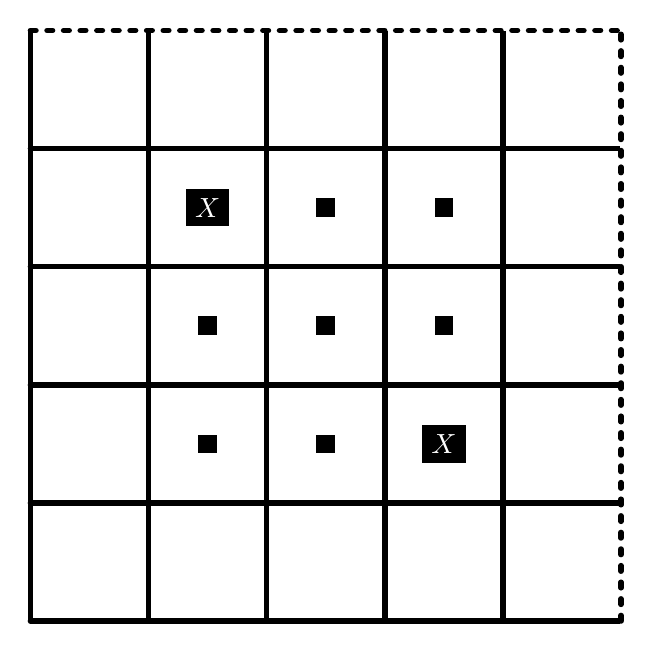
\begin{tikzpicture}[scale=0.75]
\draw[step=2, line width = 2pt, loosely dotted, line cap=round, line join=round] (0,0) grid (10,10);
\draw[step=2, line width = 2pt] (0,0) grid (9.99,9.99);
\foreach \x in {3, 5, 7}{
\foreach \y in {3, 5, 7}{
\node[fill=black] at (\x,\y){};
}
}
\foreach \x/\y/\synd in {3/7/$X$, 7/3/$X$}{
\node[fill=black] at (\x,\y){\textcolor{white}{\synd}};
}
\end{tikzpicture}
\caption{Possible $X$ syndrome pair. 
If the decoder determines that a length-4 chain exists between the two, such a path can be restricted to a bounding box whose interior is marked with black squares above. 
Only if the two syndromes are collinear is there a unique path.}
\end{figure}
\end{itemize}
We'd prefer to have a solution that can handle $Y$ errors `out of the box', to try to put them on the same footing as $X$ and $Z$. 
In the rest of this document, I loosely explore this kind of thing. 
\section{Weights}
Let's first show how the linear program for decoding syndromes independently is derived (see \cite{DKLP} for a longer and stronger explanation).
We begin by writing the probability of an $X$ error that produces pairs of $X$ syndromes, according to an independent error model:
\begin{equation}
p(E_X) = \prod_{C_X \in E_X } p^{\abs{C_X}} (1-p)^{n-\abs{C_X}},
\end{equation}
where $E_X$ is the $X$ error, $C_X$ is a continuous chain of $X$s that makes up part of the error, and $n$ is the number of qubits.
We can simplify this by taking the log: 
\begin{flalign}
p(E_X) &= (1-p)^n \prod_{C_X \in E_X } \left(\frac{p}{1-p} \right)^{\abs{C_X}}\\
& \propto \sum_{C_X \in E_X} \log \left(\frac{p}{1-p} \right)\abs{C_X} \propto -\sum_{C_X \in E_X} \abs{C_X} 
\end{flalign}
Maximizing the likelihood, then, is equivalent to minimizing the sum of lengths of the chains $C_X$ whose endpoints are given by the $X$ (or equivalently $Z$) syndromes. 

We can immediately see the problem. 
A single $Y$ error has an effective weight of two, since it is detected as a length-one $X$ chain and a length-one $Z$ chain in the absence of other errors. 
To fix this, let's make the unjustified assumption that $p_X=p_Y=p_Z$. 
They're going to be different, later (we'll actually have a very different error model later), but this is an easy place to start. 
This results in ``free edges'', since adding a $Z$ error to an edge where there's already an $X$ error results in a $Y$ error, incurring no additional cost. 
We can always adjust the costs we derive to determine how to compensate for a lower $p_Y$. 
In case of a higher $p_Y$, we can probably do a trivial code redesign to ensure that the type of error that produces excess syndromes is the least likely. 
\section{Optimisation Problem}
I'd like to have a nice structure for an optimisation problem, so I can look at slackness and adapt Blossom. 
It's not working, for the following reasons:
\subsection{Cost Not Given By Single Intersection}
In the crisp, clean picture of what these chains look like, we subtract one unit of weight whenever one chain crosses another:
\begin{figure}
[!h]
\centering
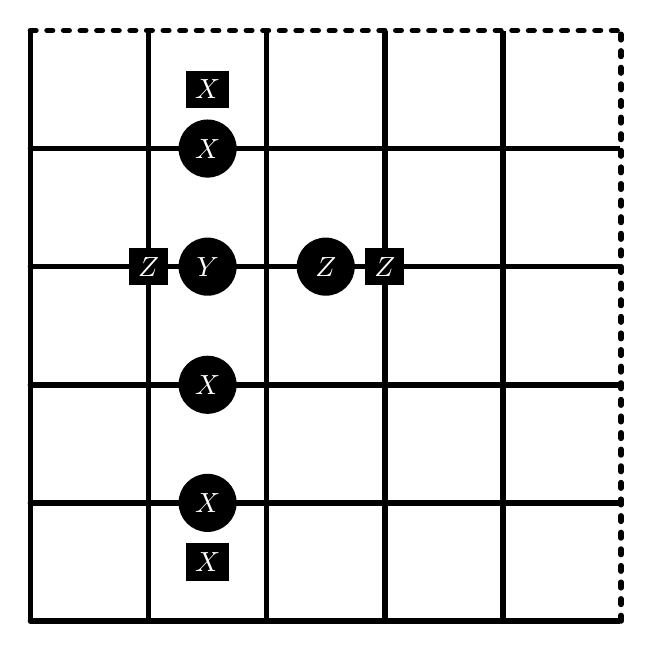
\begin{tikzpicture}[scale=0.75]
\draw[step=2, line width = 2pt, loosely dotted, line cap=round, line join=round] (0,0) grid (10,10);
\draw[step=2, line width = 2pt] (0,0) grid (9.99,9.99);
\foreach \x/\y/\err in {3/2/$X$, 3/4/$X$, 3/6/$Y$, 3/8/$X$, 5/6/$Z$}{
\fill[black] (\x,\y) circle(14pt);
\node[white] at (\x,\y){\err};
}
\foreach \x/\y/\synd in {2/6/$Z$, 6/6/$Z$, 3/1/$X$, 3/9/$X$}{
\node[fill=black] at (\x,\y){\textcolor{white}{\synd}};
}
\end{tikzpicture}
\caption{This is not a minimum-length path, but it would be on a larger lattice, so it's legitimate.}
\end{figure}

If all the chains intersected like this, we'd have a bilinear program on our hands. 
In this world, we would just record which minimum-length paths intersect in one position with which others, and evaluate the cost by pricing the $X$ and $Z$ chains separately, then evaluating a matrix element which counts the number of intersections and subtract that off. 
The first problem is that minimum-length paths which aren't straight can intersect in weird ways:
\begin{figure}
[!h]
\centering
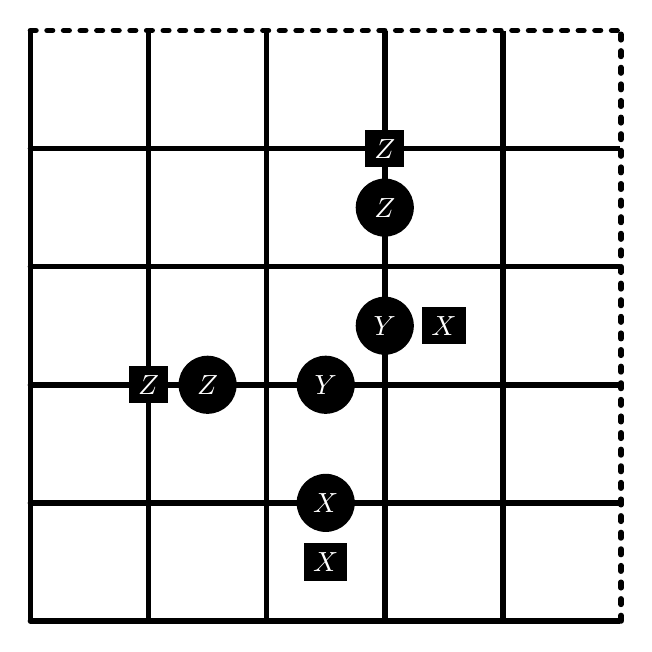
\begin{tikzpicture}[scale=0.75]
\draw[step=2, line width = 2pt, loosely dotted, line cap=round, line join=round] (0,0) grid (10,10);
\draw[step=2, line width = 2pt] (0,0) grid (9.99,9.99);
\foreach \x/\y/\err in {5/2/$X$, 5/4/$Y$, 6/5/$Y$, 6/7/$Z$, 3/4/$Z$}{
\fill[black] (\x,\y) circle(14pt);
\node[white] at (\x,\y){\err};
}
\foreach \x/\y/\synd in {7/5/$X$, 2/4/$Z$, 5/1/$X$, 6/8/$Z$}{
\node[fill=black] at (\x,\y){\textcolor{white}{\synd}};
}
\end{tikzpicture}
\caption{Bent $X$ and $Z$ paths that intersect on two qubits. Note that other minimum-length paths in the bounding boxes of these syndrome pairs can intersect on one or zero qubits.}
\end{figure}
This is in principle not a problem, since we can associate the maximum change in cost with any edge pair. 
The real problem would be if a union of three paths ($a$, $b$, and $c$) had a cost that could not be described by a bilinear function. 
\subsection{Cost Not Given By Bounding Box}
We're still trying to attach a cost to a syndrome configuration, and it looks like you can obtain this for an $X$/$Z$ pair configuration by first getting the independent cost, then counting the number of qubits where the bounding boxes of the $X$/$Z$ syndrome intersect and subtracting.
This works for the chain in Figure 6 (the bounding boxes of those syndrome pairs intersect on exactly two qubits), but it doesn't work for an arbitrary pair:
\begin{figure}[!h]
\centering
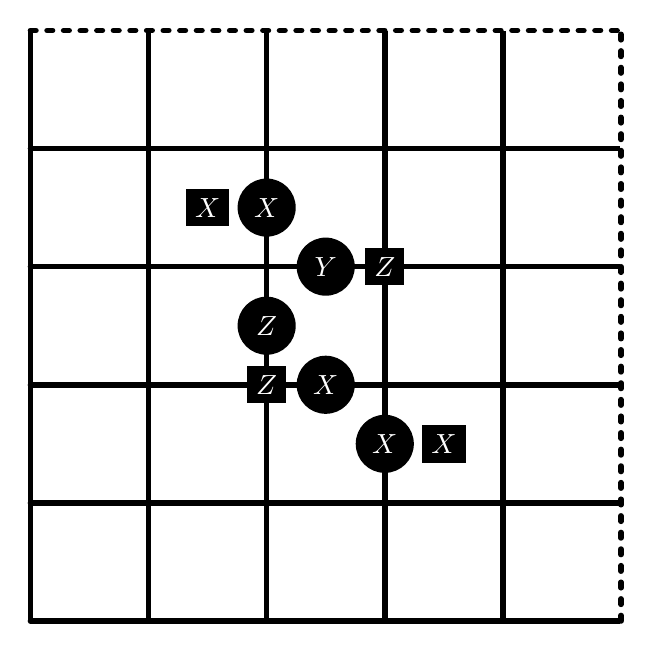
\begin{tikzpicture}[scale=0.75]
\draw[step=2, line width = 2pt, loosely dotted, line cap=round, line join=round] (0,0) grid (10,10);
\draw[step=2, line width = 2pt] (0,0) grid (9.99,9.99);
\foreach \x/\y/\err in {4/5/$Z$, 5/4/$X$, 6/3/$X$, 5/6/$Y$, 4/7/$X$}{
\fill[black] (\x,\y) circle(14pt);
\node[white] at (\x,\y){\err};
}
\foreach \x/\y/\synd in {3/7/$X$, 6/6/$Z$, 4/4/$Z$, 7/3/$X$}{
\node[fill=black] at (\x,\y){\textcolor{white}{\synd}};
}
\end{tikzpicture}
\caption{Syndrome pairs that can't be priced by bounding box intersection. 
The bounding box of the $Z$ pair is contained entirely in that of the $X$ pair, but the maximum intersection between these paths is one.}
\end{figure}
\FloatBarrier
It is now no longer clear what the cost of a syndrome should be, let alone whether it can be represented by a bilinear function.
\bibliographystyle{plain}
\bibliography{BilinearProgramForSCDecoding}
\section*{Appendices}
\appendix
\section{Measuring a Different Code Every Round}
If a bilinear program-based decoder doesn't work for whatever reason, do we have the option to measure a different set of stabilisers at every round that commute with the previous round's (e.g. CSS codes with $Y$ and $X$ strings instead of $X$ and $Z$) and reconstruct the error history from there?
A program of research suggests itself, where we go back to DKLP and figure out which errors form chains in 3D given the cycle of stabilisers that we measure. 
\section{Re-Re-weighting}
Can we solve the problem with re-weighting where a geodesic error chain is chosen arbitrarily? 
Maybe. 
We can try to evaluate the conditional probability of an $X$ error on the qubit in a syndrome pair's bounding box, given that the syndrome pair is in the matching produced by the decoder. 
We can even use message-passing to do this. 
Considering the syndrome pair in Figure 4, we take the subgraph of the dual lattice that corresponds to the bounding box:
\begin{figure}[!h]
\centering
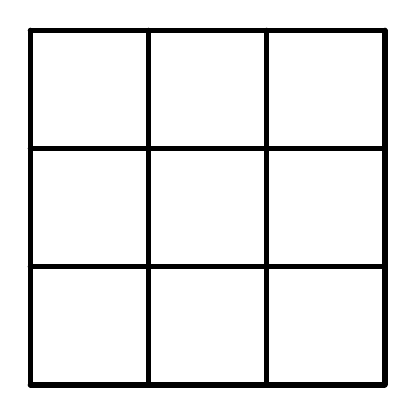
\begin{tikzpicture}[scale=0.75]
\draw[step=2, line width = 2pt, line cap=round, line join=round] (0,0) grid (6,6);
\end{tikzpicture}
\end{figure}

To ensure that we restrict to minimum-length paths, we add directions to each edge. 
We then perform a forwards and backwards pass to obtain the probability that each vertex is involved in a path:
\begin{figure}[!h]
\centering
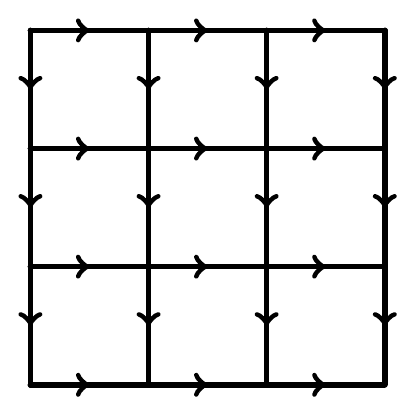
\begin{tikzpicture}[scale=0.75]
\draw[step=2, line width = 2pt, line cap=round, line join=round] (0,0) grid (6,6);
\foreach \x in {0,2,4}{
\foreach \y in {0,2,4,6}{
\draw[line width = 2pt, line cap=round, line join=round, ->] (\x,\y) --++ (1,0);
}
}
\foreach \x in {0,2,4,6}{
\foreach \y in {2,4,6}{
\draw[line width = 2pt, line cap=round, line join=round, ->] (\x,\y) --++ (0, -1);
}
}
\end{tikzpicture}
\hfill
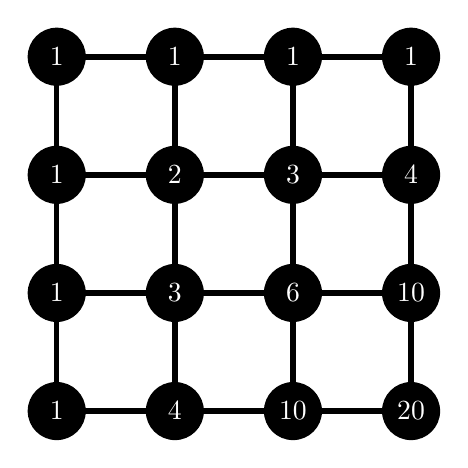
\begin{tikzpicture}[scale=0.75]
\draw[step=2, line width = 2pt, line cap=round, line join=round] (0,0) grid (6,6);
\foreach \x/\y/\num in {
0/6/1, 2/6/1, 4/6/1, 6/6/1,
0/4/1, 0/2/1, 0/0/1,
2/4/2, 4/4/3, 6/4/4,
2/2/3, 4/2/6, 6/2/10,
2/0/4, 4/0/10, 6/0/20
}{
\fill[black] (\x,\y) circle(14pt);
\node[white] at (\x,\y){$\num$};
}
\end{tikzpicture}
\hfill
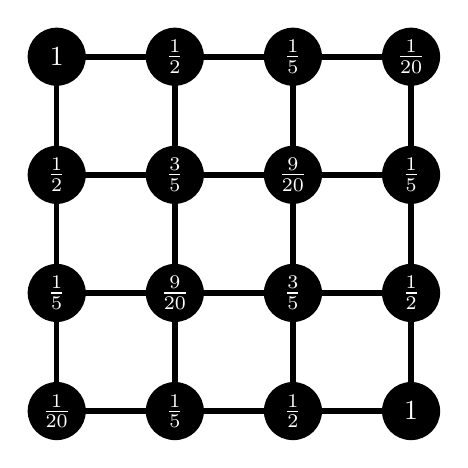
\begin{tikzpicture}[scale=0.75]
\draw[step=2, line width = 2pt, line cap=round, line join=round] (0,0) grid (6,6);
\foreach \x/\y/\f in {
0/6/1, 2/6/\frac{1}{2}, 4/6/\frac{1}{5}, 6/6/\frac{1}{20},
0/4/\frac{1}{2}, 0/2/\frac{1}{5}, 0/0/\frac{1}{20},
2/4/\frac{3}{5}, 4/4/\frac{9}{20}, 6/4/\frac{1}{5},
2/2/\frac{9}{20}, 4/2/\frac{3}{5}, 6/2/\frac{1}{2},
2/0/\frac{1}{5}, 4/0/\frac{1}{2}, 6/0/1
}{
\fill[black] (\x,\y) circle(14pt);
\node[white] at (\x,\y){$\f$};
}
\end{tikzpicture}
\caption{From left to right: Directions for which any valid path is minimum-length; number of paths from the top left to the highlighted vertex found by Pascal's triangle-type message-passing; probability of each vertex being involved in a randomly selected path.}
\end{figure}

The probability that an edge is involved in a given path is given as $p(e) = p(v_1,v_2) = p(v_1)p\left(v_2 \given v_1 \right)$, which we can evaluate by looking at subdiagrams of Figure 8:
\begin{figure}
\centering
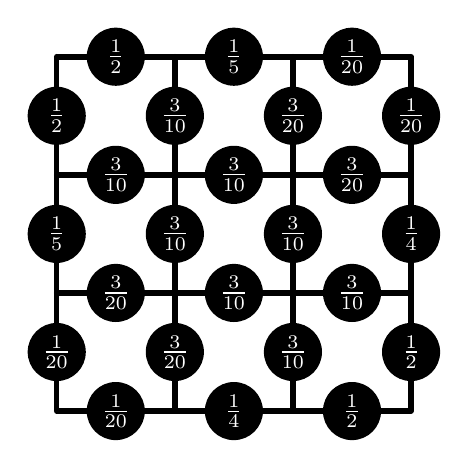
\begin{tikzpicture}[scale=0.75]
\draw[step=2, line width = 2pt, line cap=round, line join=round] (0,0) grid (6,6);
\foreach \x/\y/\f in {
1/0/\frac{1}{20}, 3/0/\frac{1}{4}, 5/0/\frac{1}{2},
0/1/\frac{1}{20}, 2/1/\frac{3}{20}, 4/1/\frac{3}{10}, 6/1/\frac{1}{2},
1/2/\frac{3}{20}, 3/2/\frac{3}{10}, 5/2/\frac{3}{10},
0/3/\frac{1}{5}, 2/3/\frac{3}{10}, 4/3/\frac{3}{10}, 6/3/\frac{1}{4},
1/4/\frac{3}{10}, 3/4/\frac{3}{10}, 5/4/\frac{3}{20},
0/5/\frac{1}{2}, 2/5/\frac{3}{10}, 4/5/\frac{3}{20}, 6/5/\frac{1}{20},
1/6/\frac{1}{2}, 3/6/\frac{1}{5}, 5/6/\frac{1}{20}
}{
\fill[black] (\x,\y) circle(14pt);
\node[white] at (\x,\y){$\f$};
}
\end{tikzpicture}
\caption{Edge probabilities obtained by evaluating conditional probabilities on sub-diagrams of Figure 8.}
\end{figure}
\FloatBarrier
Though this is a little messy, it looks like this might be a better way to re-weight the edges given that a path between the top left and bottom right corners exists. 
If it isn't, I still suspect that it's related to some way to re-weight better.
\end{document}